% Scale drives machine learning progress
\chapter{大规模数据促进机器学习发展}

\iffalse
Many of the ideas of deep learning (neural networks) have been around for decades. Why are
these ideas taking off now?
Two of the biggest drivers of recent progress have been:
• Data availability. People are now spending more time on digital devices (laptops, mobile
devices). Their digital activities generate huge amounts of data that we can feed to our
learning algorithms.
• Computational scale. We started just a few years ago to be able to train neural networks
that are big enough to take advantage of the huge datasets we now have.
In detail, even as you accumulate more data, usually the performance of older learning
algorithms, such as logistic regression, “plateaus.” This means its learning curve “flattens
out,” and the algorithm stops improving even as you give it more data:
\fi

深度学习(神经网络)的概念已经存在了数十年,
为什么现在这些概念如此流行呢?

产生近年来进步的最大两个驱动因素是:
\begin{itemize}
	\item \textbf{大量可以使用的数据}。
	人们现在越来越依赖于电子设备(笔记本,手机等等)。
	这些电子设备为我们训练算法产生了大量的数据。
	\item \textbf{大规模计算的能力}。
	我们不久前才能够训练大规模的神经网络,以利用拥有大量数据的优势。
\end{itemize}

具体地说,即使你增加更多的数据,
传统的机器学习算法的表现也会进入瓶颈,如逻辑回归。
这也就是说,它的学习曲线会趋于平坦,
学习效果甚至不会随着训练数据量的增加而变好。
\begin{figure}[h]
	\centering
	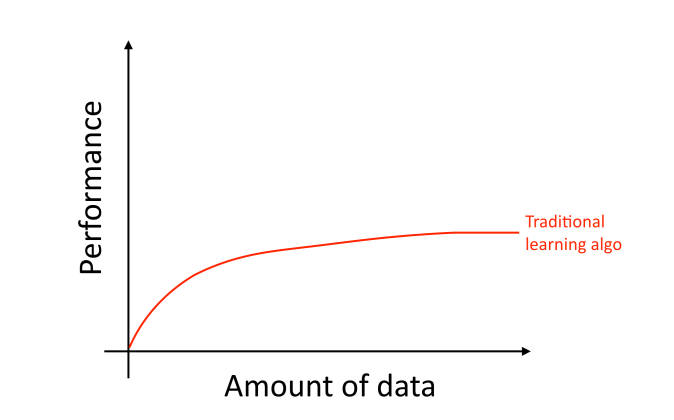
\includegraphics[width=0.5\linewidth]{TeX_files/pic/4.1}
	\caption{传统机器学习模型学习表现变化}
	\label{fig:4.1}
\end{figure}

\iffalse
It was as if the older algorithms didn’t know what to do with all the data we now have.
If you train a small neutral network (NN) on the same supervised learning task, you might
get slightly better performance:
\fi

 传统的机器学习算法并不会知道如何使用我们现在拥有的数据。
 
 如果你训练一个小的神经网络在同样的监督学习任务上,
 你会得到轻微的改善。
 \begin{figure}[h]
 	\centering
 	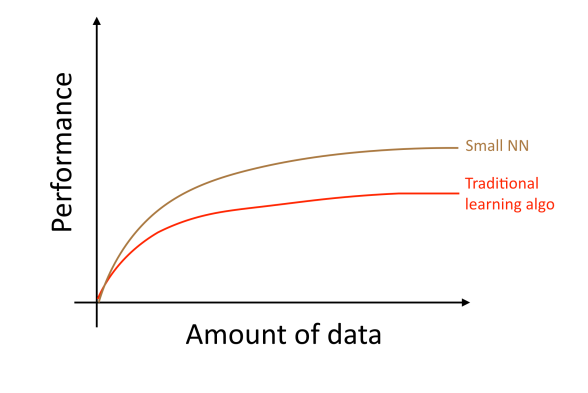
\includegraphics[width=0.7\linewidth]{TeX_files/pic/4.2}
 	\caption[神经网络的学习表现]{\footnotesize 神经网络的学习表现。这个图表展示了NN在小数据集下也会做的更好(横轴前半部分)。这和NN在大数据集中表现优秀并不具有一致性。在小数据集中,传统算法可能做得更好,也可能不会做得更好,这依赖于手工设计的特征。例如,如果你只有20个训练样本,那么你使用logistic regression 或使用neural network可能没有多大区别;手工设计的特征将会比算法的选择产生更大的影响。但是如果你拥有一百万的数据量,我更倾向于使用神经网络。}
 	\label{fig:4.2}
 \end{figure}

\iffalse
Here, by “Small NN” we mean a neural network with only a small number of hidden units/
layers/parameters. Finally, if you train larger and larger neural networks, you can obtain
even better performance:
\fi

这里的“小的神经网络”是指只有很少数量的隐藏层、节点或参数的神经网络。
最终你会发现,随着你的神经网络越来越大,
算法的表现会越来越好:

\begin{figure}[h]
	\centering
	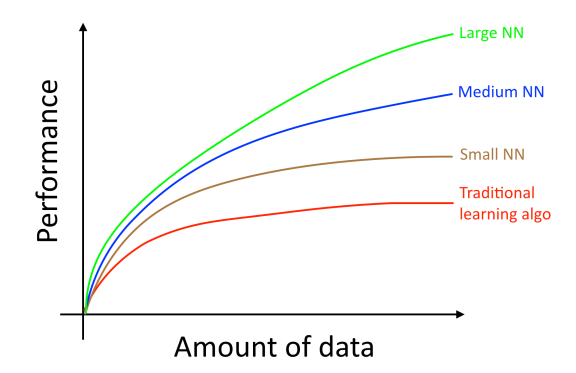
\includegraphics[width=0.4\linewidth]{TeX_files/pic/4.3}
	\caption{大规模神经网络学习表现}
	\label{fig:4}
\end{figure}


\iffalse
Thus, you obtain the best performance when you (i) Train a very large neural network, so
that you are on the green curve above; (ii) Have a huge amount of data.
Many other details such as neural network architecture are also important, and there has
been much innovation here. But one of the more reliable ways to improve an algorithm’s
performance today is still to (i) train a bigger network and (ii) get more data.
The process of how to accomplish (i) and (ii) are surprisingly complex. This book will discuss
the details at length. We will start with general strategies that are useful for both traditional
learning algorithms and neural networks, and build up to the most modern strategies for
building deep learning systems.
\fi

因此,当你(1)训练一个较大的神经网络来获得绿色的学习表现,(2)使用大量的数据时, 你会得到最好的表现。

神经网络的其他细节也同样重要,这方面有很多创新。
但是就目前来说,改善一个算法表现的主要途径还是:
(1)训练更大的神经网络,
(2)获取更多的数据。

完成上述目标的过程依然十分复杂,这本书会讨论这类细节。
我们将会从既对传统机器学习算法有用又对神经网络有用的通用策略出发,
实现对建立深度学习系统最先进的策略。

